\documentclass[french, 9pt]{article}

%-------------------------------------------------------------------------------
\usepackage[a4paper,top=1cm,bottom=2cm,left=1cm,right=1cm,marginparwidth=0.5cm]{geometry}
\usepackage{amsmath,amsfonts,amssymb,amsthm}
\usepackage[french]{babel}
\usepackage[utf8]{inputenc}
\usepackage[T1]{fontenc}
\usepackage{enumerate}
\usepackage{natbib}
\usepackage{graphicx}
\usepackage{xspace}
\usepackage{color,xcolor}
\usepackage{tikz}
\usepackage{remreset}
\usepackage{url}
\usepackage{boites}
% \usepackage{extsizes} % Permet \documentclass[french, 14pt]{extreport}
% \usepackage[a4paper,top=1cm,bottom=2cm,left=1cm,right=1cm,marginparwidth=.75cm]{geometry}
% \usepackage{minitoc}

\graphicspath{{../Figures/}}
% Environnement
\newtheorem{theorem}{Théorème}
\newtheorem{definition}{Définition}
\newtheorem{lemma}{Lemme}
\newtheorem{proposition}{Proposition}
\newtheorem*{theorem*}{Théorème}
\newtheorem*{definition*}{Définition}
\newtheorem*{proposition*}{Proposition}
\newtheorem*{corollary*}{Corollaire}
\newtheorem*{assumption*}{Hypothèse}
\newtheorem*{algorithm*}{Algorithme}
\newtheorem*{lemma*}{Lemme}
\newtheorem*{remark*}{Remarque}
\newtheorem*{exercise*}{Exercice}
\newtheorem{exercise}{Exercice}
\newcommand{\remark}{\bigskip\noindent\textbf{\textsl{Remarque.}}\xspace}
\newcommand{\remarks}{\bigskip\noindent\textbf{\textsl{Remarques.}}\xspace}
\newcommand{\parSR}[1]{\paragraph*{\textsl{#1}}\xspace}
\renewcommand{\proof}{\bigskip\noindent\underline{\textsl{Démonstration}.}\xspace}
\newcommand{\eproof}{$\blacksquare$}

% Effets, couleurs
\newcommand{\emphase}[1]{\textcolor{red}{#1}}
\newcommand{\demoProp}[1]{\noindent{\textbf{\textsl{Démonstration de la proposition \ref{#1} :}}}}
\newcommand{\itemdot}{\textbullet}

% Moments
\DeclareMathOperator{\Esp}{\mathbb{E}}
\DeclareMathOperator{\diag}{diag}
\DeclareMathOperator{\Cov}{\mathbb{C}ov}
\DeclareMathOperator{\tr}{tr}
\DeclareMathOperator{\Var}{\mathbb{V}}
\let\Pr\relax\DeclareMathOperator{\Pr}{\mathbb{P}}
\renewcommand{\d}{\text{d}}

% R, N, ...
\newcommand{\cst}{\text{cst}}
\newcommand{\Cbb}{\mathbb{C}}
\newcommand{\Ibb}{\mathbb{I}}
\newcommand{\Nbb}{\mathbb{N}}
\newcommand{\Rbb}{\mathbb{R}}
\newcommand{\Zbb}{\mathbb{Z}}

% Indicateurs

% Lois et ensembles
\newcommand{\Acal}{\mathcal{A}}
\newcommand{\Bcal}{\mathcal{B}}
\newcommand{\Ccal}{\mathcal{C}}
\newcommand{\Ecal}{\mathcal{E}}
\newcommand{\Gcal}{\mathcal{G}}
\newcommand{\Ical}{\mathcal{I}}
\newcommand{\Lcal}{\mathcal{L}}
\newcommand{\Mcal}{\mathcal{M}}
\newcommand{\Ncal}{\mathcal{N}}
\newcommand{\Pcal}{\mathcal{P}}
\newcommand{\Rcal}{\mathcal{R}}
\newcommand{\Scal}{\mathcal{S}}
\newcommand{\Ucal}{\mathcal{U}}
\newcommand{\Xcal}{\mathcal{X}}
\newcommand{\Ycal}{\mathcal{Y}}

% Comments
\newcommand{\SR}[2]{\textcolor{gray}{#1}\textcolor{red}{#2}}
\newcommand{\todo}[1]{\textcolor{red}{\`A faire~: {\sl #1}}}
\newcommand{\dessin}[1]{
\begin{center}\framebox{\begin{minipage}{\textwidth}
  \textcolor{purple}{#1}
\end{minipage}}\end{center}
\bigskip
}
\newcommand{\progres}[1]{
\begin{center}\framebox{\begin{minipage}{\textwidth}
  \textcolor{blue}{{\sl #1}}
\end{minipage}}\end{center}
\bigskip
}
\newcommand{\solution}[1]{
\begin{center}\framebox{\begin{minipage}{\textwidth}
  \noindent{\sl Solution :}
  #1
\end{minipage}}\end{center}
\bigskip
}
% \newcommand{\exemple}[1]{
% \begin{center}\framebox{\begin{minipage}{\textwidth}
%   \parSR{Exemple.}
%   #1
% \end{minipage}}\end{center}
% \bigskip
% }
\newcommand{\exemple}[1]{
\begin{breakbox}
  \parSR{Exemple.}
  #1
\end{breakbox}
\bigskip
}

\newcommand{\SRcorrect}[2]{\textcolor{gray}{#1}\textcolor{blue}{#2}}
\newcommand{\SRcomment}[1]{\textcolor{blue}{[{\sl SR: #1}]}}



% Section numbering
\usepackage{chngcntr}
\renewcommand{\thepart}{\Roman{part}}
% \counterwithout{section}{part}
\setcounter{secnumdepth}{3}
\setcounter{tocdepth}{1}

% Proposition numbering
\renewcommand{\subsubsection}{\section}
% \numberwithin{exercise}{section}
% \numberwithin{equation}{section}

% Suppression des solutions
\renewcommand{\solution}[1]{}

\newcommand{\alglin}{/home/robin/ENSEIGN/Cours/MathBiologie/L3-ENS-Math1/Exercices/AlgLin}
\newcommand{\multivar}{/home/robin/ENSEIGN/Cours/MathBiologie/L3-ENS-Math1/Exercices/MultiVar}
\newcommand{\equadiff}{/home/robin/ENSEIGN/Cours/MathBiologie/L3-ENS-Math1/Exercices/EquaDiff}
\newcommand{\probas}{/home/robin/ENSEIGN/Cours/MathBiologie/L3-ENS-Math1/Exercices/Probas}


% %-------------------------------------------------------------------------------
% %-------------------------------------------------------------------------------
% \title{\Huge{Ce qu'un biologiste doit savoir en mathématiques}}
% \author{SR d'après \cite{Lam20} : Annexes}
% \date{\today}


\title{\normalsize{\sc École Normale Supérieure de Paris, Licence de Biologie L3}
  
  \bigskip
  \normalsize{\sc Année 2025–25}
  
  \bigskip
  \large{\bf Mathématiques I : ce qu’un biologiste ne doit pas ignorer} 
  
}
\date{Examen, le XX janvier 2025}

%-------------------------------------------------------------------------------
%-------------------------------------------------------------------------------
\begin{document}
%-------------------------------------------------------------------------------
%-------------------------------------------------------------------------------

\maketitle

\bigskip
L'épreuve dure 2 heures. 
Les notes de cours individuelles sont autorisées.
L’usage de tout appareil électronique est interdit à l’exception d’une calculatrice.

%-------------------------------------------------------------------------------
% \section{Algèbre linéaire}
% %-------------------------------------------------------------------------------
\subsubsection{Dynamique d'une population de Leslie}
%-------------------------------------------------------------------------------

% Cf exercice 5 AL

On considère une population structurée en $n$ classes d'âge. Pour $1 \leq i \leq n$, on note $x_k(t)$ le nombre d'individus de la classe $k$ à la génération $t$ et $x(t) = [x_1(t) \dots x_n(t)]^\top$ le vecteur décrivant l'ensemble de la population à cette même génération. On suppose que l'évolution de cette population est régit par la récurrence
\begin{equation} \label{eq:recurrenceLeslie}
  x(t+1) = A x(t)
\end{equation}
où $A$ est la matrice de Leslie
$$
A = \left[\begin{array}{cccccc}
            f_1 & f_2 & \cdots  & \cdots & f_n \\
            s_1 & 0 & \cdots  & \cdots & 0 \\
            0 & \ddots  & \ddots & & \vdots \\
            \vdots & \ddots & \ddots & \ddots & \vdots \\
            0 & \cdots & 0 & s_{n-1} & 0 \\
          \end{array}\right]
$$
où tous les coefficients $f_i$ et $s_i$ sont supposés strictement positifs. On note de plus
$$
\ell_1 = 1 \qquad \text{et} \qquad 
\ell_k = \prod_{i=1}^{k-1} s_i \quad \text{pour $2 \leq k \leq n$}.
$$

\begin{enumerate}
  \item Interprêter les coefficients $f_i$ et $s_i$.
  \solution{$f_i$ est le taux de fertilité de la classe $i$ (qui alimente la classe 1). $S_i$ est le taux de survie de la classe $i$ (qui alimente la classe $i+1$).}
  %
  \item Soient $B_{k1} \in \Mcal_{k-1}$, $B_{k2} \in \Mcal_{n-k}$ définies par :
  $$
  B_{k1} = \left[\begin{array}{cccc}
            s_1 & -\lambda & &  \\
            & \ddots & \ddots & \\
            & & \ddots & -\lambda \\
            & & & s_{k-1}
          \end{array}\right], \qquad
  B_{k2} = \left[\begin{array}{cccc}
            -\lambda & & & \\
            s_{k+1} & \ddots & & \\
            & \ddots & \ddots & \\
            & & s_{n-1} & -\lambda
          \end{array}\right].
  $$
  En notant $0_{p,q}$ la matrice $p \times q$ dont tous les éléments sont nuls, calculer le déterminant de la matrice $B_k \in \Mcal_{n-1}$ :
  $$
  B_k = \left[\begin{array}{cc}
            B_{k1} & 0_{k-1, n-k} \\
            0_{n-k, k-1} & B_{k2}
          \end{array}\right].
  $$
  \solution{On utilise le calcul du déterminant par bloc pour obtenir
  $$
  |B| = |B_{k1}| \times |B_{k2}|
  $$
  et on remarque que, puisque $B_{k1}$ et $B_{k2}$ sont respectivement triangulaires supérieure et inférieure, leurs déterminants sont égaux au produit de leurs termes diagonaux, soit
  $$
  |B_{k1}| = \ell_k, \qquad |B_{k2}| = (-\lambda)^{n-k}.
  $$
  }
  %
  \item Montrer que le polynôme caractéristique de $A$ est
  $$
  P_A(\lambda) = (f_1 - \lambda) (-\lambda)^{n-1} + \sum_{k=2}^{n} (-1)^{k-1} f_k \ell_k (-\lambda)^{n-k}.
  $$
  \solution{Les termes successifs du développement du déterminant 
  $$
  |A - \lambda I| 
  = \left|\begin{array}{cccccc}
            f_1-\lambda & f_2 & \cdots  & \cdots & f_n \\
            s_1 & -\lambda & 0  & \cdots & 0 \\
            0 & s_2 & \ddots & \ddots & \vdots \\
            \vdots & \vdots & \ddots & \ddots & 0 \\
            0 & \cdots & 0 & s_{n-1} & -\lambda \\
          \end{array}\right|
  $$ 
  par rapport à la première ligne sont
  \begin{align*}
  (f_1 - \lambda) |B_1| & = (f_1-\lambda) (-\lambda^{n-1}), &
  - f_2 |B_2| & = -f_2 s_1 (-\lambda)^{n-2}, \\
  f_3 |B_3| & = f_3 s_1 s_2 (-\lambda)^{n-3}, & 
  -f_4 |B_4| & = -f_4 s_1 s_2 s_3 (-\lambda)^{n-4}, \qquad \dots
  \end{align*}
  }
  %
  \item En déduire que la plus grande valeur propre en module $\lambda_1$ de la matrice $A$ vérifie
  $$
  \sum_{k=1}^n \ell_k f_k \lambda_1^{-k} = 1.
  $$
  \solution{Toutes les valeurs propres, dont $\lambda_1$, sont solutions de $P_A(\lambda) = 0$, soit
  \begin{align*}
  (f_1 - \lambda) (-\lambda)^{n-1} + \sum_{k=2}^{n} (-1)^{k-1} f_k \ell_k (-\lambda)^{n-k} & = 0 \\
  \Leftrightarrow \qquad \sum_{k=1}^n (-1)^{k-1} f_k \ell_k (-\lambda)^{n-k} & = (-\lambda)^{n-1} & 
  \Leftrightarrow \qquad \sum_{k=1}^n f_k \ell_k \lambda^k & = 1.
  \end{align*}
  }
\end{enumerate}

On s'intéresse maintenant aux vecteurs propres à gauche et à droite de la matrice $A$. On note 
$$
a = \sum_{k=1}^n \ell_k \lambda_1^{-k}, \qquad
b = \sum_{k=1}^n k \ell_k f_k \lambda_1^{-k}.
$$
\begin{enumerate}
  \setcounter{enumi}{4}
  \item Montrer que le vecteur $v$ de coordonnées
  $$
  v_k = \frac1a \ell_k \lambda_1^{-k}, \qquad 1 \leq k \leq n,
  $$
  est un vecteur propre à droite de $A$ associé à la valeur propre $\lambda_1$.
  \solution{Soit le vecteur $w = Av$. Ses coordonnées sont
  \begin{align*}
    w_1 & = \sum_{k=1}^n f_k v_k = \frac1a \sum_{k=1}^n f_k \ell_k \lambda_1^{-k} = \frac1a = \lambda_1 v_1, \\
    w_k & = s_{k-1} v_{k-1} = \frac1a s_{k-1} \ell_{k-1} \lambda_1^{-k+1}  = \frac1a \ell_k \lambda_1^{-k+1} = \lambda_1 v_k, \qquad \text{pour $2 \leq k \leq n$}.
  \end{align*}
  }
  \item Montrer que le vecteur $u$ de coordonnées
  $$
  u_k = \frac1{b v_k} \sum_{j=k}^n \ell_j f_j \lambda_1^{-j}, \qquad 1 \leq k \leq n,
  $$
  est un vecteur propre à gauche de $A$ associé à la valeur propre $\lambda_1$.
  \solution{Soit le vecteur $w^\top = u^\top A$. On a
  $$
  w_n = f_n u_1
    = f_n \frac{a \lambda_1}b \sum_{j=1}^n \ell_j f_j \lambda_1^{-j}
    = f_n \frac{a \lambda_1}b
  $$
  or
  $$
  u_n = \frac{\ell_n f_n \lambda_1^{-n}}{b v_n} = \frac{a f_n}{b}, 
  \qquad \text{donc} \quad w_n = \lambda_1 u_n.
  $$
  De plus, pour $1 \leq k \leq n-1$, on a
  \begin{align*}
    w_k & = f_k u_1 + s_k u_{k+1} 
    = f_k \frac{a \lambda_1}{b} \sum_{j=1}^n \ell_j f_j \lambda_1^{-j} + s_k \frac{a \lambda_1^{k+1}}{b \ell_{k+1}} \sum_{j=k+1}^n \ell_j f_j \lambda_1^{-j} \\
    & = \frac{a \lambda_1^{k+1}}{b \ell_k} \left(f_k \ell_k \lambda_1^{-k} + \sum_{j=k+1}^n \ell_j f_j \lambda_1^{-j}\right)
    = \lambda_1 \frac{a \lambda_1^k}{b \ell_k} \sum_{j=k}^n \ell_j f_j \lambda_1^{-j}
    = \lambda_1 u_k.
  \end{align*}}
\end{enumerate}

On s'intéresse enfin au comportement asymptotique du vecteur $x(t)$ décrivant la composition de la population au bout de $t$ générations.
\begin{enumerate}
  \setcounter{enumi}{6}
  \item Calculer $\sum_{k=1}^n v_k$ et $\sum_{k=1}^n v_k u_k$.
  \solution{On a
  \begin{align*}
    \sum_{k=1}^n v_k 
      & = \frac1a \sum_{k=1}^n \ell_k \lambda_i^{-k} = 1 \\
    \sum_{k=1}^n v_k u_k 
      & = \frac1b \sum_{k=1}^n \sum_{j=k}^n \ell_j f_j \lambda_1^{-j}
      = \frac1b \sum_{k=1}^n k \ell_k f_k \lambda_1^{-k} = 1.
  \end{align*}}
  \item Partant d'un vecteur de composition initial $x(0)$, quel est le comportement asymptotique de $x(t)$ quand $t$ tend vers l'infini ?
  \solution{La récurrence \eqref{eq:recurrenceLeslie} implique que $x(t) = A^t x(0)$. De plus, le théorème de Perron-Frobénius nous assure que $\lim_{t \to \infty} \lambda_1^{-t} A^t = v u^\top$. On a donc
  $$
  \lim_{t \to \infty} \lambda_1^{-t} x(t) 
  = \lim_{t \to \infty} \lambda_1^{-t} A^t x_0(t)
  = v u^\top x(0) = \left(u^\top x(0)\right) v
  $$
  soit $x(t) \approx c_0 \lambda_1^t v$, avec $c_0 = u^\top x(0)$.
  \begin{itemize}
   \item La taille totale de la population évolue asymptotiquement comme $\lambda_1^n$. 
   \item La composition asymptotique relative de la population est donnée par les coordonnées du vecteur $v$ (qui somment à 1). 
   \item Le produit scalaire $c_0$ indique comment les effectifs initiaux $x_k(0)$ contribuent respectivement (à proportion de $u_k$) à la taille asymptotique de la population.
  \end{itemize}}
\end{enumerate}


%-------------------------------------------------------------------------------
% \section{Fonction de plusieurs variables}
% %-------------------------------------------------------------------------------
\subsubsection{Exemple de fonction de $\Rbb^2 \mapsto \Rbb$}
%-------------------------------------------------------------------------------

Soit la fonction $f: \Rbb^2 \mapsto \Rbb$ définie par
$$
f(x, y) = x^3 + y^3 - 3 xy
$$

\begin{enumerate}
  \item Déterminer les points stationnaires de la fonction $f$.
  \solution{
    Le gradient de $f$ vaut
    $$
    \nabla f = \left[\begin{array}{c} 3x^2 - 3y \\ 3y^2 - 3x \end{array}\right]
    $$
    qui est nul aux points
    $$
    a = (0, 0) \qquad \text{et} \qquad b = (1, 1).
    $$
  }
  \item Déterminer s'il s'agit de maximums, de minimums ou de points selles.
  \solution{
    La hessienne vaut
    $$
    \nabla^2 f = \left[\begin{array}{rrr} 6x & & -3 \\ -3 & & 6y \end{array}\right].
    $$
    \begin{description}
      \item[\'Etude du point $a$ :] on a 
      $$
      \nabla_a^2 f = \left[\begin{array}{rrr} 0 & & -3 \\ -3 & & 0 \end{array}\right]
      \qquad \Rightarrow \qquad 
      | \nabla_a^2 f | = -9 < 0
      $$
      donc $a$ est un point selle. Ses valeurs propres sont les racines de
      $$
      P(\lambda) = \left|\begin{array}{rrr} -\lambda & & -3 \\ -3 & & -\lambda \end{array}\right|
      = \lambda^2 - 9 
      \qquad \text{soit} \quad 
      \lambda = \pm 3.
      $$
      Tout vecteur propre associé à $\lambda = -3$ est solution de 
      $$
      \left\{\begin{array}{rcl} -3y & = & -3x \\-3x & = & -3y\end{array} \right.
      \qquad \Rightarrow \qquad 
      x = y
      \qquad \Rightarrow \qquad 
      \left[ \begin{array}{r} 1 \\ 1 \end{array} \right] \text{ est associé à $-3$}
      $$
      donc $a$ est un maximum dans la direction de la 1ère bissectrice. \\
      Tout vecteur propre associé à $\lambda = 3$ est solution de 
      $$
      \left\{\begin{array}{rcl} -3y & = & 3x \\-3x & = & 3y\end{array} \right.
      \qquad \Rightarrow \qquad 
      x = -y
      \qquad \Rightarrow \qquad 
      \left[ \begin{array}{r} -1 \\ 1 \end{array} \right] \text{ est associé à $+3$}
      $$
      donc $a$ est un minimum dans la direction de la 2ème bissectrice.
      $$
      \begin{tabular}{cc}
        direction $x = y$ & direction $x = -y$ \\
        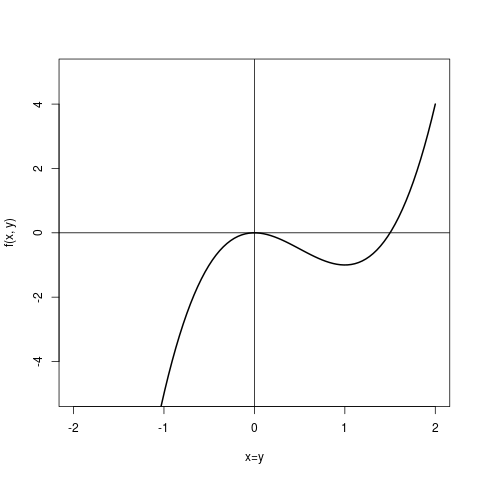
\includegraphics[width=.35\textwidth, trim=00 10 10 40, clip=]{ExempleOptimum-1ereBissectrice} &
        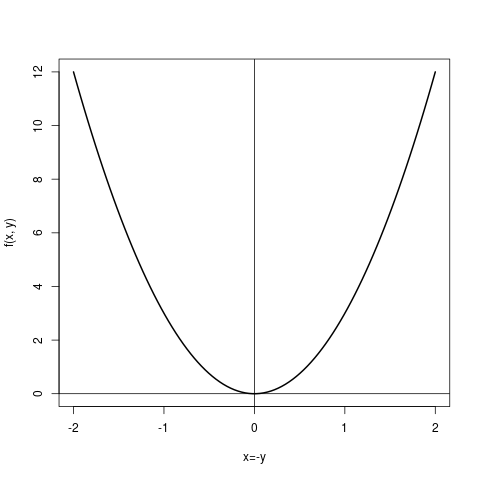
\includegraphics[width=.35\textwidth, trim=00 10 10 40, clip=]{ExempleOptimum-2emeBissectrice} \\
        $f(x, x) = 2x^3 - 3x^2$ & $f(x, -x) = 3x^2$
      \end{tabular}
      $$
      \item[\'Etude du point $b$ :] on a
      $$
      \nabla_b^2 f = \left[\begin{array}{rrr} 6 & & -3 \\ -3 & & 6 \end{array}\right]
      \qquad \Rightarrow \qquad 
      | \nabla_b^2 f | = 27 > 0, \qquad \tr(\nabla_b^2 f) = 12 > 0
      $$
      donc les deux valeurs propres de $\nabla_b^2 f$ sont positives : $b$ est donc un minimum.
    \end{description}
    Au total la surface d'équation $\{z = f(x, y)\}$ a l'aspect suivant
    $$
    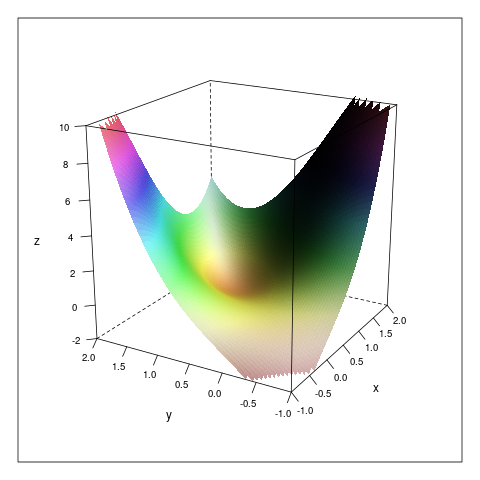
\includegraphics[width=.6\textwidth]{ExempleOptimum-surface}
    $$
  }
\end{enumerate}


%-------------------------------------------------------------------------------
% \section{Systèmes dynamiques}
\bigskip \bigskip 
%-------------------------------------------------------------------------------
\subsubsection{Système de Lorenz en 2 dimensions} 
%-------------------------------------------------------------------------------

On considère une version réduite à deux dimensions du système de Lorenz, c'est-à-dire à un couple $(x(t), y(t))_{t \geq 0}$ satisfaisant les conditions initiales
$$
x(0) = x_0, \qquad y(0) = y_0
$$
et vérifiant le système d'équations différentielles ordinaires
\begin{equation*} % \label{eq:lorenz2D}
  \left\{\begin{array}{rcl}
    \dot x & = a x - xy \\
    \dot y & = x^2 - by
  \end{array}\right.
\end{equation*}
où les coefficients $a$ et $b$ sont strictement positifs.

\paragraph{Détermination des points stationnaires et de leur stabilité.}
\begin{enumerate}
  \item Montrer que le système admet trois points stationnaires.
  \solution{
    En annulant simultanément
    $$
    F_1(x, y) = a x - xy, \qquad F_2(x, y) = x^2 - by,
    $$
    on détermine que le vecteur gradient est nul aux points 
    $$
    O = (0, 0), \qquad A = (\sqrt{ab}, a) \quad \text{et} \quad B = (-\sqrt{ab}, a).
    $$
  }
  \item Déterminer la matrice Jacobienne du système.
  \solution{
  On a
  $$
  J f = \left[\begin{array}{cc} a-y & -x \\ 2x & -b \end{array} \right].
  $$
  }
  \item En déduire la nature (stable ou instable) de chacun des points stationnaires.
  \solution{
  \begin{description}
    \item[$O = (0, 0)$ :] On a
    $$
    J_0 f = \left[\begin{array}{cc} a & 0 \\ 0 & -b \end{array} \right],
    $$
    dont les valeurs propres ($\lambda_1 = a, \lambda_2 = b)$ sont de signes opposés : $O$ est donc instable. Plus précisément, il est instable le long de l'axe des $x$ et stable le long de l'axe des $y$.
    \item[$A = (\sqrt{ab}, a)$ :] On a
    $$
    J_A f = \left[\begin{array}{cc} 0 & -\sqrt{ab} \\ 2\sqrt{ab} & -b \end{array} \right],
    $$
    donc $\tr(J_A f) = -b < 0$ et $\det(J_A f) = 2ab > 0$. Les deux valeurs propres sont donc de même signe et négatives : $A$ est donc un équilibre stable. \\
    {\sl Alternative :} Le polynôme caractéristique
    $$
    P_A(\lambda) = \lambda^2 + b \lambda + 2 ab
    $$
    a pour discriminant $\Delta = b^2 - 8 ab$. 
    \begin{itemize}
      \item Si $0 < a < b/8$, $\Delta$ est positif et les valeurs propres sont 
      $$
      \lambda_1 = \frac12 \left(-b + \sqrt{\Delta}\right) 
      \quad \text{et} \quad
      \lambda_2 = \frac12 \left(-b - \sqrt{\Delta}\right).
      $$
      comme de plus $\Delta < b^2$, les deux valeurs propres sont négatives, donc $A$ est stable.
      \item Si $a > b/8$, $\Delta$ est négatif et les valeurs propres sont 
      $$
      \lambda_1 = \frac12 \left(-b + i \sqrt{|\Delta|}\right) 
      \quad \text{et} \quad
      \lambda_2 = \frac12 \left(-b - i \sqrt{|\Delta|}\right),
      $$      
      dont la partie entière commune est $-b < 0$, donc $A$  est également stable.
    \end{itemize}
    \item[$B = (-\sqrt{ab}, a)$ :] On a alors    
    $$
    J_B f = \left[\begin{array}{cc} 0 & \sqrt{ab} \\ -2\sqrt{ab} & -b \end{array} \right]
    $$
    qui a la même trace et le même déterminant que $J_A f$ : $B$ est donc également stable. \\
    {\sl Alternative :} Le polynôme caractéristique de $J_B f$ est le même que celui de $J_A f$ donc $B$ est de même nature que $A$.
  \end{description}
  }
\end{enumerate}

\paragraph{Cas de paramètres négatifs.}
On étudie maintenant le cas où les paramètres $a$ et $b$ peuvent prendre des valeurs négatives. On ne s'attardera pas sur les cas limites $a = 0$ et/ou $b = 0$.

\bigskip
\begin{enumerate}
  \setcounter{enumi}{3}
  \item Déterminer le ou les points stationnaires et étudier sa (leur) stabilité quand $a$ est négatif ($b$ étant toujours strictement positif).
  \solution{
    Si $a < 0$ (et $b > 0$), alors $ab < 0$ donc $O$ est le seul point stationnaire, et les deux valeurs propres de $J_O f$ sont négatives, donc $O$ est stable.
  }
  \item Mener la même étude pour $a > 0$ et $b < 0$, d'une part, et pour $a < 0$ et $b < 0$, d'autre part.
  \solution{
  \begin{description}
    \item[$a > 0, b < 0$ :] Alors $ab < 0$ donc $O$ est le seul point stationnaire, mais les deux valeurs propres de $J_O f$ sont positives, donc $O$ est instable. 
    \item[$a < 0, b < 0$ :] Alors $ab > 0$ donc $O$, $A$ et $B$ sont stationnaires.
    \begin{itemize}
      \item Le valeurs propres de $J_O f$ sont alors de signes opposés, donc $O$ est instable.
      \item On a $\tr(J_A f) = \tr(J_B f) = -b > 0$ et $\det(J_A f) = \det(J_B f) = 2 ab > 0$. Les deux valeurs propres sont donc positives et $A$ et $B$ sont donc instables. \\
      {\sl Alternative:} Le discriminant de $P_A(\lambda)$ (et donc de $P_B(\lambda)$) vaut alors $\Delta = b^2 - 8ab > b^2 > 0$. Les deux valeurs propres
      $$
      \lambda_1 = \frac12 \left(-b + \sqrt{\Delta}\right) 
      \quad \text{et} \quad
      \lambda_2 = \frac12 \left(-b - \sqrt{\Delta}\right).
      $$
      sont alors de signe opposé : $A$ et $B$ sont donc instables.
    \end{itemize}
  \end{description}
  }
\end{enumerate}



%-------------------------------------------------------------------------------
% \section{Probabilités}
\bigskip \bigskip 
%-------------------------------------------------------------------------------
\subsection{Modèle d'apparition de tumeurs}
%-------------------------------------------------------------------------------

% Inspiré du modèle d'apparition des tumeurs CDH1 de type II, avec A. Bonnet
% https://www.overleaf.com/project/61fa6f1f2e1b2e66da2e825b
% Transféré dans /home/robin/Bureau/RECHERCHE/GENETIQUE/CDH1/Doc/CDH1_Poisson
% ATTENTION : chgt de notation ! \pi(t) -> 1 - \pi(t).

\paragraph{Modèle.}
On considère l'apparition de tumeurs malignes en deux étapes:
\begin{enumerate}
  \item les tumeurs de type B (bénignes) apparaissent selon un processus de Poisson homogène d'intensité constante $\lambda$ et
  \item chaque tumeur de type B se transforme ensuite en une tumeur de type M (maligne) au bout d'un temps exponentiel de paramètre $\mu$ (donc d'espérance $1/\mu$).
\end{enumerate}

On note $N(t)$ le nombre total de tumeurs apparues au temps $t$ : 
$$
\{N(t)\}_{t \geq 0} \sim PP(\lambda t).
$$
et $M(t)$ le nombre de tumeurs de type M au temps $t$. Le nombre de tumeurs bénignes au temps $t$ vaut donc $B(t) = N(t) - M(t)$.

\bigskip
\paragraph{Question préliminaire.}
\begin{enumerate}
  \item Montrer que si $X$ suit une loi de Poisson $\Pcal(\alpha)$ et que $Y$ sachant $X=x$ suit un loi binomiale $\Bcal(x, p)$, alors $Y$ suit une loi de Poisson $\Pcal(\alpha p)$.
  \solution{
  On intègre la loi conditionnelle de $Y \mid X$ par rapport à la loi de $X$, soit : 
  \begin{align*}
    \Pr\{Y = y\}
    & 
    = \sum_{x \geq y} \Pr\{Y = y \mid X = x\} \Pr\{X = x\}
    = \sum_{x \geq y} \left(\begin{array}{c}x \\ y \end{array}\right) p^y (1-p)^{x-y}e^{-\alpha} \frac{\alpha^x}{x !} \\
    &
    = e^{-\alpha} \sum_{x \geq y} \left(\begin{array}{c}x \\ y \end{array}\right) (\alpha p)^y (\alpha - p)^{x-y} {x !} 
    = e^{-\alpha} \frac{(\alpha p)^y}{y !} \sum_{x \geq y} \frac1{(x - y) !}(\alpha - \alpha p)^{x-y}. 
  \end{align*}
  En posant $z = x-y$, on reconnaît
  $$
  \sum_{x \geq y} \frac1{(x - y) !} (\alpha - \alpha p)^{x-y} 
  =
  \sum_{z \geq 0} \frac1{z !}(\alpha - \alpha p)^{z} 
  =
  e^{\alpha p - \alpha},
  $$
  soit finalement
  $$
  \Pr\{Y = y\}
  = e^{-\alpha} \frac{(\alpha p)^y}{y !} e^{\alpha p - \alpha}
  = e^{-\alpha p} \frac{(\alpha p)^y}{y !}
  $$
  où on reconnaît la loi de Poisson $\Pcal(\alpha p)$. 
  \paragraph{\sl Alternative.} On peut aussi se souvenir que la fonction génératrice de la loi de Poisson vaut $\phi_X(s) = e^{\alpha(s-1)}$ et que celle de la loi de Bernoulli est $\phi_Z(s) = 1 -p + ps$. Puisque $Y$ est la somme de $X$ variables aléatoires de Bernoulli (de paramètre $p$) indépendantes, sa fonction génératrice vaut 
  $
  \phi_Y(s) 
  = \phi_X \circ \phi_Z(z)
  = \exp(\alpha(-p + ps)) 
  = \exp(\alpha p (s - 1)),
  $
  qui est la fonction génératrice de la loi de Poisson $\Pcal(\alpha p)$.
  }
\end{enumerate}


\bigskip
\paragraph{Loi du nombre de tumeurs de type B.}
On s'intéresse d'abord à l'apparition des tumeurs et au temps durant lequel elle restent de type $B$.

\bigskip
\begin{enumerate}
  \setcounter{enumi}{1}
  \item Donner la loi du nombre total $N(t)$ de tumeurs au temps $t$.  
  \solution{
  C'est une des propriétés du processus de Poisson: $N(t) \sim \Pcal(\lambda t)$.
  }
  %
  \item Donner la probabilité qu'une tumeur de type B apparue au temps $s$ soit toujours de type B au temps $t > s$.
  \solution{
  Les tumeurs de type B se transforment en tumeurs de type M au bout d'une durée exponentielle de paramètre $\mu$. Une telle durée dépasse $u$ avec probabilité $e^{-\mu u}$, la probabilité demandée vaut donc
  $e^{-\mu (t-s)}$.
  }  
  %
  \item Montrer que la probabilité qu'une tumeur de type B apparue avant $t$ soit toujours de type B au temps $t > s$ vaut
  $$
  \pi(t) = \frac1{\mu t} (1 - e^{-\mu t}).
  $$
  \solution{
  D'après une autre propriété du processus de Poisson, sachant qu'une tumeur est apparue avant $t$, sa date d'apparition $T$ est distribuée uniformément sur l'intervalle $[0, T]$ (et sa densité vaut donc $1/t$ partout entre $0$ et $t$). La probabilité demandée vaut donc
  \begin{align*}
    \int_0^t \frac1t e^{-\mu (t-s)} \; \d s
    = \frac1t e^{-\mu t} \int_0^t e^{\mu s} \; \d s
    = \frac1t e^{-\mu t} \frac1\mu (e^{\mu t} - 1)
    = \frac1{\mu t} (1 - e^{-\mu t}).
  \end{align*}
  La figure suivante donne $\pi(t)$ pour $\lambda = 1$ et \textcolor{red}{$\mu = 1/8$}, \textcolor{green}{$\mu = 1/4$}, \textcolor{blue}{$\mu = 1/2$} et \textcolor{cyan}{$\mu = 1$}.
  $$
  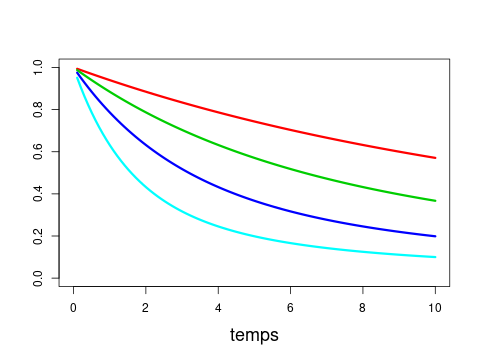
\includegraphics[width=0.5\textwidth, trim=20 40 20 50, clip=]{TumeurCDH1-ProbaApparition}
  $$
  }  
%   \begin{figure}
%     \begin{center}
%     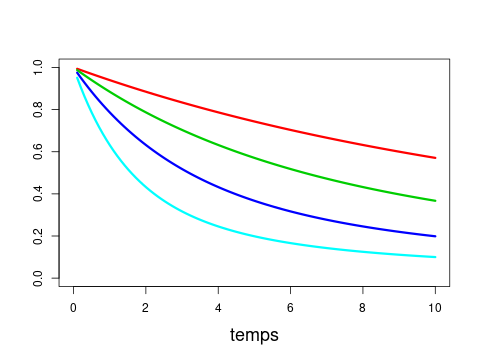
\includegraphics[width=0.5\textwidth, trim=20 40 20 50, clip=]{TumeurCDH1-ProbaApparition}
%     \caption{Probabilité $\phi(t)$ pour $\lambda = 1$ et \textcolor{red}{$\mu = 1/4$}, \textcolor{green}{$\mu = 1/2$} et \textcolor{blue}{$\mu = 1$}.}
%     \end{center}
%   \end{figure}
  %
\end{enumerate}

\bigskip
\paragraph{Loi du nombre de tumeurs de type M.}
On s'intéresse maintenant à la vitesse d'apparition des tumeurs de type M.

\bigskip
\begin{enumerate}
  \setcounter{enumi}{4}
  \item Donner la loi du nombre $M(t)$ de tumeurs de type M sachant le nombre total $N(t)$ de tumeurs apparues avant $t$ est égale à $n$: $N(t) = n$.
  \solution{
  Conditionnellement au fait que $n$ tumeurs sont apparues au temps $t$, chacune d'entre elle est encore de type B avec probabilité $\pi(t)$ et est donc de type M avec probabilité $1 - \pi(t)$. Ces tumeurs étant apparues et s'étant transformées indépendamment, le nombre de tumeurs de type M au temps $t$ suit une loi binomiale :
  $$
  \left(M(t) \mid N(t) = n\right) \sim \Bcal(n, 1 - \pi(t)).
  $$
  \paragraph{\sl Alternative.} On peut aussi reprendre le calcul de la question précédente en intégrant simultanément sur les temps d'apparition $s_1 \dots s_n$ des $n$ cellules présentes et en distinguant celles qui sont restées de type B (avec probabilité $e^{-\mu(t - s)}$) de celles qui se sont transformées en cellules de type M (avec probabilité $1 - e^{-\mu(t - s)}$). On écrit ainsi $\Pr\{M(t) = m \mid N(t) = n\}$
  \begin{align*}
    & = \idotsint_{[0, t]^n} \binom{n}{m} \prod_{j=1}^m \frac1t \underset{\text{passée en type M}}{\underbrace{(1- e^{-\mu(t-s_j)})}} \d s_j \prod_{k=m+1}^{n} \frac1t \underset{\text{toujours de type B}}{\underbrace{e^{-\mu(t-s_k)}}} \d s_k \\
    & = \binom{n}{m} \prod_{j=1}^m \left(\frac1t \int_{[0, t]} (1- e^{-\mu(t-s_j)}) \d s_j \right) \prod_{k=m+1}^{n} \left(\frac1t \int_{[0, t]} e^{-\mu(t-s_k)} \d s_k\right) \\
%     & = \binom{n}{m} \left(1 -e^{-\mu t} \left[\frac{e^{\mu t}-1}{\mu}\right]\right)^m  \left( e^{-\mu t} \left[\frac{e^{\mu t}-1}{\mu}\right]\right)^{n-m} \\
    &= \binom{n}{m} \left(1- \frac{1 - e^{-\mu t}}{\mu t}\right)^m \left( \frac{1 - e^{-\mu t}}{\mu t}\right)^{n-m}
  \end{align*}
  où on reconnait une loi binomiale :
  $$
  \left(M(t) \mid N(t) = n\right) \sim \Bcal(n, 1 - \pi(t)).
  $$
  }
  %
  \item En déduire la loi du nombre $M(t)$ de tumeurs de type M apparues avant $t$.
  \solution{
  On applique le résultat de la question préliminaire avec $X = N(t)$, $\alpha = \lambda t$, $Y = M(t)$ et $p = 1 - \pi(t)$ pour obtenir que le nombre de tumeurs de type M au temps $t$ suit une loi de Poisson :
  $$
  M(t) \sim \Pcal\left(\lambda t [1 - \pi(t)]\right).
  $$
  }
  %
  \item Donner la probabilité qu'aucune tumeur de type M ne soit apparue au temps $t$.
  \solution{
  Puisque la probabilité qu'une variable de Poisson de paramètre $m$ soit nulle vaut $e^{-m}$, on a 
  $$
  \Pr\{M(t) = 0\} 
  = \exp\left(- \lambda t [1 - \pi(t)]\right)
  = \exp\left(- \lambda \left[t - \frac{1 - e^{-\mu t}}{\mu}\right]\right)
  $$
  La figure suivante donne $\Pr\{M(t) = 0\}$ pour $\lambda = 1$ et \textcolor{red}{$\mu = 1/8$}, \textcolor{green}{$\mu = 1/4$}, \textcolor{blue}{$\mu = 1/2$} et \textcolor{cyan}{$\mu = 1$}. 
  La courbe noire donne la probabilité d'absence de toute tumeur : $\Pr\{N(t) = 0\} = e^{-\lambda t}$.
  $$
  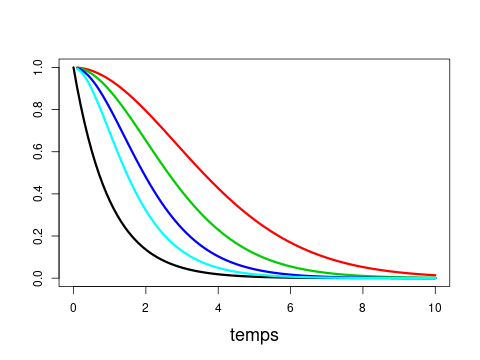
\includegraphics[width=0.5\textwidth, trim=20 40 20 50, clip=]{TumeurCDH1-ProbaAbsence}
  $$
  }
  %
  \item On suppose qu'en moyenne un tumeur bénigne apparaît chaque année et que chacune d'elle devient maligne en moyenne au bout de cinq ans. Calculer la probabilité qu'aucune tumeur maligne ne soit apparue au bout de dix ans.
  \solution{
  Le paramètres sont alors $\lambda = 1$, $\mu = 1/5$ et $t = 10$, qui donne
  $\Pr\{M(t) = 0\} = 0.0034 = 0.34\%$.
  }
\end{enumerate}



%-------------------------------------------------------------------------------
%-------------------------------------------------------------------------------
\end{document}
%-------------------------------------------------------------------------------
%-------------------------------------------------------------------------------


